%%
% 第三章节
\chapter{模型结构}

本章介绍语音情绪识别系统中使用的主要模型结构。经过信号处理阶段获得的 log-Mel 谱图、梅尔频率倒谱系数、韵律特征等输入表示，能够将情绪相关的声学线索整理为固定格式，但要从这些表示中判别实际情绪类别，需要合适的模型结构\cite{ma2023review,lin2023chunk}。在语音情绪识别中，模型设计涉及分类器选择的问题，同时也涉及如何学习输入特征的结构特性与时间依赖关系。

本章首先介绍语音情绪识别的基础神经网络模型结构，随后依次介绍注意力机制与 Transformer 模型。3.1 节说明全连接神经网络模型、卷积神经网络模型、循环神经网络模型及其典型变体，总结这些结构在语音情绪识别中的作用与局限。3.2 节阐述注意力机制，3.3 节介绍 Transformer 模型及其主要原理。上述介绍可为理解本研究所用模型结构提供基础。


\section{现有基础模型结构}


\subsection{全连接神经网络模型}

全连接神经网络（Fully Connected Neural Network，也称多层感知机MLP）是基本的人工神经网络模型，每一层的每个神经元与下一层的所有神经元相互连接。在语音情绪识别早期研究中，通常将人为设计特征（梅尔频率倒谱系数、基频、能量等）组织为固定长度向量并输入该模型完成分类\cite{ma2023review}。单层的输出表示为：
\begin{equation}
\mathbf{h}^{(l)} = \phi \left( \mathbf{W}^{(l)} \mathbf{h}^{(l-1)} + \mathbf{b}^{(l)} \right)
\end{equation}
其中$\mathbf{W}^{(l)}$为权重矩阵，$\mathbf{b}^{(l)}$为偏置，$\phi(\cdot)$为非线性激活函数。输出层采用softmax将logit转换为类别概率，训练时采用交叉熵损失。全连接神经网络模型难以保留语音信号中的时间结构与局部空间结构，适合处理发话级汇总特征，在直接学习时频结构方面相对受限\cite{peng2021efficient,zhang2023cnn}。

\begin{figure}[!htbp]
    \centering
    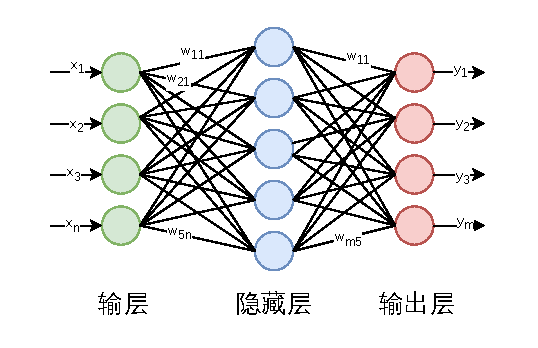
\includegraphics[width=0.45\textwidth]{images/feedback_diagrams/chapter3/mlp/mlp.drawio (1).pdf}
    \caption{全连接神经网络模型的基本层级连接结构}
    \label{fig:mlp_neural_network}
\end{figure}

图\ref{fig:mlp_neural_network}给出了全连接神经网络模型的基本结构。图中的圆形节点表示神经元，箭头表示相邻层之间的全连接映射。输入层接收固定长度特征向量，隐藏层形成中间表示，输出层用于生成类别预测。

\subsection{卷积神经网络模型}

卷积神经网络模型是一种专门用于学习输入数据局部模式的神经网络结构。在图像处理领域，卷积神经网络模型被广泛应用。在语音情绪识别中，卷积神经网络模型同样适用于分析语音的时频表示\cite{peng2021efficient}。在语音情绪识别中，log-Mel谱图、梅尔频率倒谱系数图、谱图等二维输入表示较为常用。卷积神经网络模型可提取log-Mel谱图、梅尔频率倒谱系数图、谱图等二维输入表示中的局部时频模式。例如，卷积神经网络模型可自动学习特定频带的能量集中、短时内的强度变化以及局部频谱纹理差异\cite{zhang2023cnn}。

\begin{figure}[htbp]
    \centering
    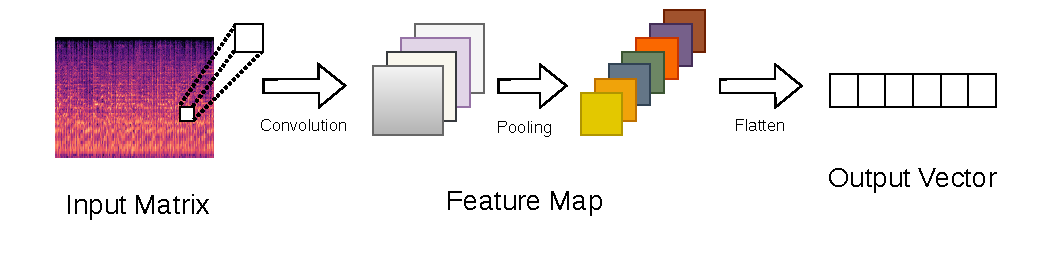
\includegraphics[width=0.68\textwidth]{images/feedback_diagrams/chapter3/cnn/cnn.drawio.pdf}
    \caption{卷积神经网络在对数梅尔谱图上通过卷积核、特征图和池化提取局部时频模式}
    \label{fig:cnn_local_feature_extraction}
\end{figure}

图\ref{fig:cnn_local_feature_extraction}将二维对数梅尔谱图视为输入矩阵，展示卷积核在局部区域内提取模式、形成特征图并经过池化压缩的过程。该过程对应语音情绪识别中对局部频带纹理、短时能量变化和相邻时间帧关系的建模。

卷积神经网络模型的主要运算是卷积。对于二维输入特征图 $\mathbf{X}$ 与卷积核 $\mathbf{K}$，输出特征图中一个位置的计算方式为：
\begin{equation}
y_{i,j}^{(k)} = \sum_{m=0}^{M-1}\sum_{n=0}^{N-1} w_{m,n}^{(k)} \, x_{i+m,j+n} + b^{(k)} 
\end{equation}
其中 $x_{i+m,j+n}$ 为输入特征图的值，$w_{m,n}^{(k)}$ 为第 $k$ 个卷积核的权重，$b^{(k)}$ 为偏置，$y_{i,j}^{(k)}$ 为输出特征图在位置 $(i,j)$ 的值，$M, N$ 为卷积核尺寸。

卷积后通常使用非线性激活函数，如 ReLU：
\begin{equation}
\text{ReLU}(x) = \max(0, x) 
\end{equation}

为降低维度和增强平移不变性，常使用池化操作。例如最大池化：
\begin{equation}
p_{i,j}^{(k)} = \max_{(m,n)\in \Omega_{i,j}} y_{m,n}^{(k)}
\end{equation}
其中 $\Omega_{i,j}$ 为池化窗口区域。卷积神经网络模型的特性包括参数共享和局部连接。同一卷积核在输入的不同位置重复使用，有助于使卷积神经网络模型的参数数量少于全连接神经网络模型，并可用于学习局部模式\cite{peng2021efficient}。

在语音情绪识别中，卷积神经网络模型具有以下优势。第一，能够捕捉谱图或对数梅尔谱图中的局部能量结构与纹理。第二，参数共享机制使得在有限数据条件下可获得一定的泛化能力。第三，通过堆叠多个卷积层，可逐步从低级特征学习到高级语义特征\cite{peng2021efficient,zhang2023cnn}。

卷积神经网络模型存在一定局限性。卷积操作主要在局部感受野内学习模式, 难以建模发话过程中的长期依赖关系或全局上下文\cite{liu2023dualrobustness}. 此外, 反复使用池化操作可能降低时间分辨率. 若情绪线索分布在发话中相距较远的多个片段之间, 仅依靠卷积神经网络模型可能不足以充分表示. 一些语音情绪识别研究将卷积神经网络模型与循环神经网络、注意力机制或Transformer模型结合, 以补充长期上下文信息\cite{chen2023dwformer}.


\subsection{循环神经网络模型及其变体}

循环神经网络模型可视为一种为建模时间序列数据的顺序结构而设计的神经网络模型。全连接神经网络模型和卷积神经网络模型能够处理输入的静态结构或局部模式，循环神经网络模型则相对有利于反映时间点之间的依赖关系和顺序信息\cite{ma2023review}。在语音情绪识别中，情绪可能通过发话过程中的基频轮廓变化、能量轮廓的上升与下降、停顿与发音模式的累积效应等表现出来。时间序列建模具有一定作用\cite{lin2023chunk}。

\begin{figure}[htbp]
    \centering
    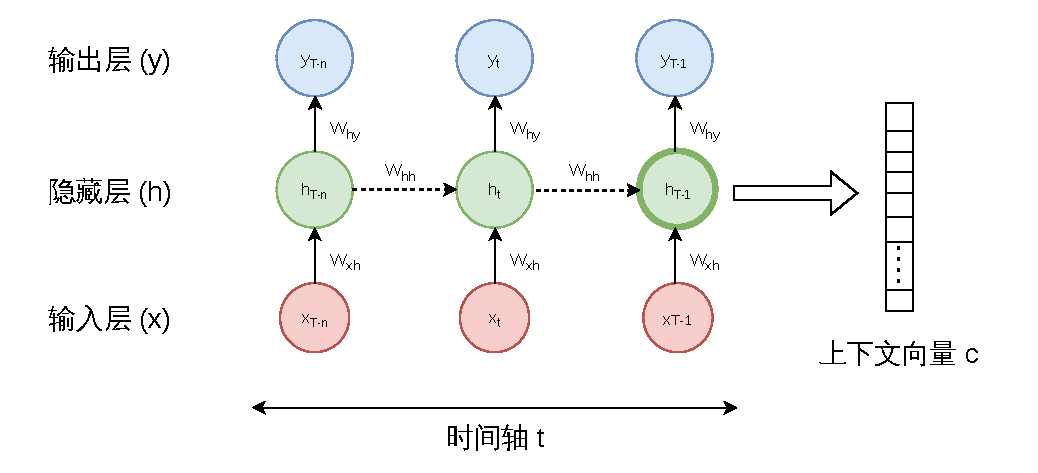
\includegraphics[width=0.68\textwidth]{images/feedback_diagrams/chapter3/rnn/rnn.drawio.pdf}
    \caption{循环神经网络沿时间帧递推隐藏状态并形成发话级上下文表示}
    \label{fig:rnn_sequence_context}
\end{figure}

图\ref{fig:rnn_sequence_context}把语音帧序列表示为按时间递推的输入，隐藏状态在相邻时刻之间传递。同时在序列末端形成用于分类的上下文表示。该结构说明循环神经网络模型为何适合描述发话过程中的顺序变化。

基本循环神经网络模型的隐藏状态更新可表示为：
\begin{equation}
\mathbf{h}_t = \phi(\mathbf{W}_{xh}\mathbf{x}_t + \mathbf{W}_{hh}\mathbf{h}_{t-1} + \mathbf{b}_h)
\end{equation}
其中 $\mathbf{x}_t$ 为 $t$ 时刻的输入向量，$\mathbf{h}_{t-1}$ 为上一时刻的隐藏状态，$\phi(\cdot)$ 为激活函数。在处理长序列时，循环神经网络模型可能出现梯度消失问题。长短期记忆网络（LSTM）通过遗忘门 $\mathbf{f}_t$、输入门 $\mathbf{i}_t$、输出门 $\mathbf{o}_t$ 与细胞状态 $\mathbf{c}_t$ 的门控机制缓解该问题\cite{lin2023chunk}：
\begin{align}
\mathbf{c}_t &= \mathbf{f}_t \odot \mathbf{c}_{t-1} + \mathbf{i}_t \odot \tanh(\mathbf{W}_c[\mathbf{h}_{t-1}, \mathbf{x}_t] + \mathbf{b}_c) \\
\mathbf{h}_t &= \mathbf{o}_t \odot \tanh(\mathbf{c}_t)
\end{align}
其中 $\odot$ 为逐元素乘法，各门均由 sigmoid 函数与线性变换构成。门控循环单元（GRU）将遗忘门与输入门合并为更新门 $\mathbf{z}_t$，并引入重置门 $\mathbf{r}_t$，结构相对简洁\cite{lin2023chunk}。双向长短期记忆网络同时处理正向与反向序列，将两方向隐藏状态拼接后用于发话级表示，能够利用发话前后的上下文，在相关研究中得到应用\cite{zhang2023cnn,lin2023chunk}。

循环神经网络模型存在一定局限。第一，顺序计算结构可能导致并行效率相对较低，在处理较长序列时计算成本可能增加。第二，长短期记忆网络模型和门控循环单元模型缓解了基本循环神经网络模型的长期依赖问题。在极长序列中，循环神经网络模型难以充分覆盖部分关键区间。第三，对于发话中哪些区间对情绪判断更为关键，循环神经网络模型缺乏选择性强调的机制。


\section{注意力机制}

在语音情绪识别中, 有研究指出情绪信息可能以不均匀的方式分布于整个发话, 相对集中于特定的时间区间、特定的频率范围或特定的声学模式之中\cite{mirsamadi2017automatic,liu2023discriminative,zou2022speech,he2023multiple}. 卷积神经网络模型和循环神经网络模型可用于学习语音表示；在采用统一权重处理输入各部分时，模型可能难以充分区分与情绪判断相关性相对较高的区间\cite{zhang2023cnn,liu2023dualrobustness,peng2021efficient}. 注意力机制作为一种计算输入内部相关性并据此调整信息组合权重的结构方法，被引入语音情绪识别中. 注意力机制通过相关性计算与加权聚合来重新分配信息重要性，既包括基于查询、键、值计算输入元素之间关系的注意力结构，也包括根据查询与键-值来源不同区分的自注意力和交叉注意力；根据注意力分数的计算方式，可使用缩放点积注意力或加性注意力；根据结构的并行化或作用范围，可使用多头注意力或局部注意力等扩展形式\cite{chen2023dwformer,wang2024swin}.


本节首先介绍注意力机制的基本概念与关键要素，说明查询、键、值的含义以及自注意力与交叉注意力的区别。随后介绍两种典型的注意力分数计算方法：缩放点积注意力和加性注意力。然后讨论多头注意力和局部注意力等结构扩展方式。最后总结注意力机制在语音情绪识别中的作用，并讨论其在数据规模、计算复杂度和可解释性等方面的局限。


\begin{figure}[htbp]
    \centering
    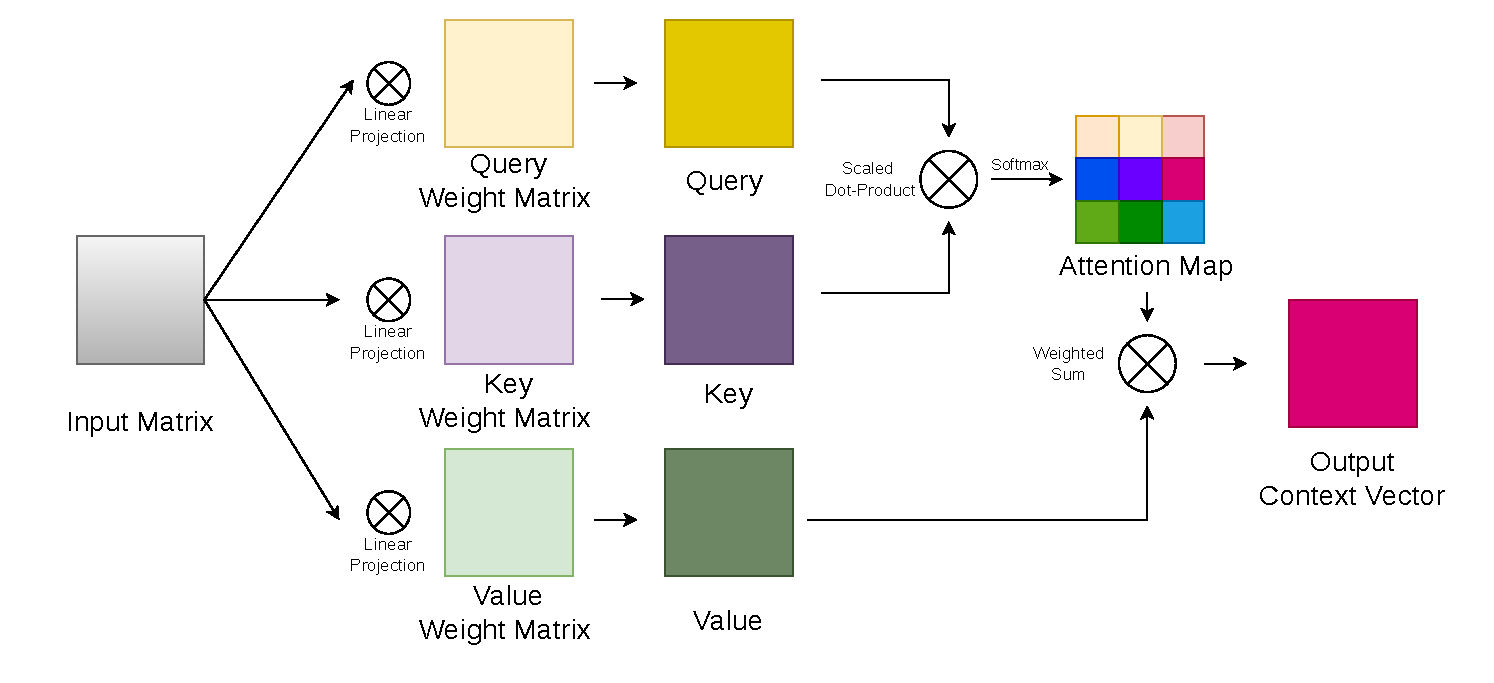
\includegraphics[width=0.65\textwidth]{images/feedback_diagrams/chapter3/attention/self_attention.drawio.pdf}
    \caption{注意力机制通过查询、键和值计算相关性权重并突出关键语音片段}
    \label{fig:attention_qkv_weighting}
\end{figure}

图\ref{fig:attention_qkv_weighting}以输入表示到查询、键和值的投影为主线，展示相关性得分、归一化权重和加权求和之间的关系。对语音情绪识别任务该图对应模型从发话中筛选相对高相关片段的过程。

\subsection{注意力机制的基本概念与关键要素}

注意力机制可理解为一种计算输入序列或特征图中各元素之间相关性，并根据计算结果调整信息组合权重的通用方法\cite{mirsamadi2017automatic,zou2022speech}。在语音情绪识别中，情绪线索并非均匀分布于整个发话，通常相对集中于特定时间区间、特定频率范围或特定声学模式\cite{liu2023discriminative,he2023multiple}。基于这一特性，注意力机制通过计算输入内部元素之间的关联程度，并据此重新分配信息重要性，从而更有选择性地反映与情绪判断相关性较高的区间。

在注意力计算过程中，首先需要定义用于量化各输入元素之间相关性的注意力分数。设输入序列中第 $i$ 个元素与第 $j$ 个元素的相关性得分为 $e_{ij}$，注意力机制通常对这些得分进行归一化后计算加权和。该过程的一般形式可表示为：
\begin{equation}
e_{ij} = a(q_i, k_j)
\label{eq:attn_general_score}
\end{equation}

\begin{equation}
\alpha_{ij} = \frac{\exp(e_{ij})}{\sum_{j'=1}^{T}\exp(e_{ij'})}
\label{eq:attn_general_alpha}
\end{equation}

\begin{equation}
z_i = \sum_{j=1}^{T}\alpha_{ij} v_j
\label{eq:attn_general_output}
\end{equation}
其中 $a(\cdot,\cdot)$ 为相关性计算函数，$q_i$、$k_j$、$v_j$ 分别表示查询、键和值，$e_{ij}$、$\alpha_{ij}$ 和 $z_i$ 分别表示注意力分数、归一化权重和注意力输出。不同注意力形式的主要差异在于相关性函数 $a(\cdot,\cdot)$ 的定义方式\cite{chen2023dwformer,wang2024swin,he2023multiple}。

在注意力计算中，查询、键、值是常用的基本元素。设输入表示为矩阵 $X$，注意力机制通常从 $X$ 或不同输入表示构造查询矩阵 $Q$、键矩阵 $K$、值矩阵 $V$，并计算它们之间的相关性。基础的线性变换形式可表示为：
\begin{equation}
Q = X_Q W_Q,\qquad K = X_K W_K,\qquad V = X_V W_V
\label{eq:qkv_linear_general}
\end{equation}
其中 $X_Q$、$X_K$、$X_V$ 分别为用于生成查询、键、值的输入表示，$W_Q$、$W_K$、$W_V$ 为可学习的权重矩阵。当三者来自同一输入时，注意力用于计算单一输入内部的元素关系。三者来源不同时，则用于计算不同表示之间的交互关系\cite{chen2023dwformer,wang2024swin,he2023multiple}。

根据查询、键、值的来源，注意力可分为自注意力和交叉注意力。自注意力是指查询、键、值均来自同一输入表示的结构。其一般形式可写为：
\begin{equation}
Q = XW_Q,\qquad K = XW_K,\qquad V = XW_V
\label{eq:self_qkv}
\end{equation}
\begin{equation}
\mathrm{SelfAttention}(X) = \mathrm{Attention}(Q,K,V)
\label{eq:self_attention}
\end{equation}
其中 $X$ 为一个输入序列或时频特征表示。自注意力用于计算同一输入内部各位置之间的相关性，可反映特定时间帧与其他帧之间的情绪关联\cite{mirsamadi2017automatic,zou2022speech,chen2023dwformer}。

交叉注意力则是指查询与键-值对来自不同输入表示（$Q=XW_Q$，$K=YW_K$，$V=YW_V$，$X$与$Y$为不同输入），用于建模不同特征空间之间的交互关系\cite{zou2022speech,he2023multiple}。



% 3.2.2
\subsection{代表性的注意力分数计算方式}
注意力可视为将输入元素之间的相关性量化为注意力分数，并通过归一化形成加权和的机制。注意力分数的计算方式是决定注意力行为特性的关键因素。当前较为常用的注意力分数计算方法主要包括缩放点积注意力和加性注意力。两种方法均通过查询与键之间的相关性计算分数，但在分数计算函数的结构与特性上存在差异\cite{vaswani2017attention,mirsamadi2017automatic,chen2023dwformer,wang2024swin}。

缩放点积注意力基于查询与键的点积计算注意力分数。设输入序列中第 $i$ 个查询为 $q_i$，第 $j$ 个键为 $k_j$，则注意力分数可表示为：
\begin{equation}
e_{ij} = \frac{q_i k_j^\top}{\sqrt{d_k}}
\label{eq:scaled_dot_score}
\end{equation}
其中 $q_i k_j^\top$ 为查询与键的点积，$d_k$ 为键向量的维度。除以 $\sqrt{d_k}$ 的原因在于：随着维度增加，点积值的方差可能增大，从而导致 softmax 输出趋于极端分布。缩放点积注意力中的缩放因子可视为提高学习稳定性的修正项\cite{vaswani2017attention,chen2023dwformer,wang2024swin}。

计算得到的分数在后续步骤中仍通过 softmax 归一化形成注意力权重，并与值向量加权聚合，其过程与式 \eqref{eq:attn_general_alpha} 和式 \eqref{eq:attn_general_output} 所示的一般形式一致。缩放点积注意力的矩阵形式可表示为：
\begin{equation}
\mathrm{Attention}(Q,K,V) = \mathrm{softmax}\left(\frac{QK^\top}{\sqrt{d_k}}\right)V
\label{eq:scaled_dot_attention_matrix}
\end{equation}
其中 $QK^\top$ 表示查询矩阵与键矩阵之间的点积结果，$\sqrt{d_k}$ 为缩放因子。该形式将分数计算、归一化与加权聚合统一为矩阵运算\cite{vaswani2017attention,chen2023dwformer,wang2024swin}。

\begin{figure}[htbp]
    \centering
    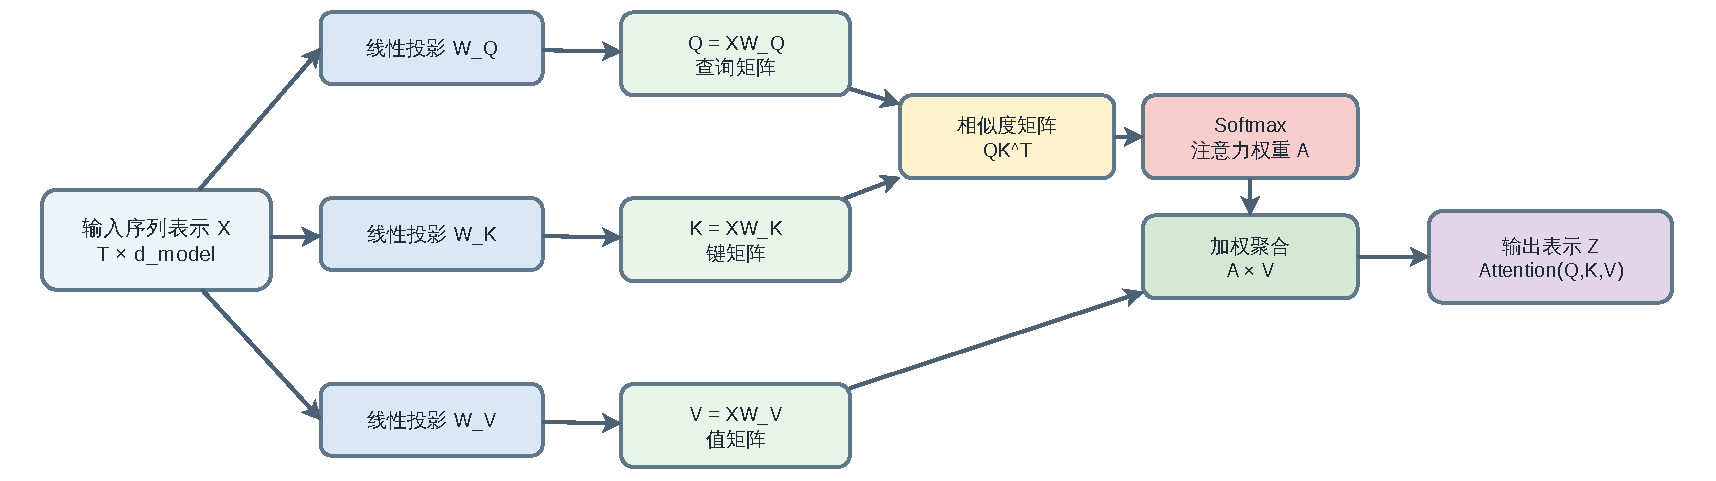
\includegraphics[width=0.68\textwidth]{images/chapter3/chapter3_attention_qkv.drawio.pdf}
    \caption{缩放点积注意力中的查询、键、值计算流程}
    \label{fig:chapter3_attention_qkv}
\end{figure}

图\ref{fig:chapter3_attention_qkv}对应式\ref{eq:scaled_dot_attention_matrix}中的矩阵计算流程。输入序列先经线性投影生成查询矩阵、键矩阵和值矩阵。以后由查询与键计算注意力权重。最后用该权重对值矩阵进行加权聚合。

缩放点积注意力基于矩阵乘法，较适合并行计算。在语音情绪识别中，该结构可用于反映特定时间帧或局部区域与其他位置之间的情绪相关性\cite{vaswani2017attention,he2023multiple}。

加性注意力通过非线性变换计算分数，不使用查询与键的点积。其一般形式可表示为：
\begin{equation}
e_{ij} = v_a^\top \tanh(W_q q_i + W_k k_j + b_a)
\label{eq:additive_attention_score}
\end{equation}
其中 $W_q$ 和 $W_k$ 分别为查询与键的权重矩阵，$b_a$ 为偏置向量，$v_a$ 为用于计算最终分数的可学习向量。该方法先对查询与键进行线性变换，再通过非线性函数得到分数\cite{mirsamadi2017automatic}。

加性注意力在归一化与加权聚合阶段仍遵循式 \eqref{eq:attn_general_alpha} 和式 \eqref{eq:attn_general_output}，主要差异集中在分数构造方式上\cite{mirsamadi2017automatic}。


% 3.2.3
\subsection{注意力的结构类型与扩展方式}

在实际应用中，注意力机制的结构设计需考虑单次注意力运算的并行化方式，以及计算范围是全局还是局部。多头注意力和局部注意力保持原有的注意力分数计算方式，是对已计算注意力的扩展，分别将注意力应用于不同的表示空间或不同的计算范围\cite{vaswani2017attention,chen2023dwformer,wang2024swin,mirsamadi2017automatic}。

仅使用单头注意力时，输入内部的各种关系需要在同一个权重结构中得到反映，此时可能难以充分分离不同类型的信息。为缓解上述问题，研究者们提出了多头注意力\cite{vaswani2017attention,chen2023dwformer,wang2024swin}。多头注意力将单次注意力运算并行化为多个头部，使模型能够在不同的表示子空间中同时学习多种类型的关系。

设头部数量为 $h$，第 $i$ 个头部可表示为：
\begin{equation}
\mathrm{head}_i = \mathrm{Attention}(QW_i^Q,\; KW_i^K,\; VW_i^V)
\label{eq:multihead_head}
\end{equation}
其中 $W_i^Q$、$W_i^K$、$W_i^V$ 分别为第 $i$ 个头部对应的查询、键、值变换矩阵。各头部使用不同的权重矩阵，即使输入表示相同，也能从不同角度学习相关性。所有头部的输出经拼接后，再通过一次线性变换得到最终结果：
\begin{equation}
\mathrm{MultiHead}(Q,K,V) = \mathrm{Concat}(\mathrm{head}_1,\mathrm{head}_2,\ldots,\mathrm{head}_h)W^O
\label{eq:multihead_output}
\end{equation}
其中 $W^O$ 为输出变换矩阵。该结构使模型能够并行反映比单头注意力更多类型的关系\cite{vaswani2017attention,chen2023dwformer,wang2024swin}。

在语音情绪识别中，情绪线索可能出现在语调变化、能量分布、频率结构、长期上下文等多个层面，也可能存在于单一维度。基于情绪线索的多维特性，部分头部可能对语调变化或能量分布较为敏感，另一些头部则可能更关注频率结构或长期上下文关系。多头注意力可用于同时反映语音信号中的多层次情绪线索\cite{he2023multiple,chen2023dwformer,wang2024swin,hou2022multi}。

多头注意力在能够处理更多关系的同时，头部数量的增加也可能导致参数数量和计算量相应上升。在数据规模有限的条件下，增加头部数量不一定带来性能提升，模型复杂度的增加可能对泛化能力造成一定负担\cite{chen2023dwformer,wang2024swin,lin2023chunk,gao2024adversarial,ahn2025multitask}。在语音情绪识别中，需要结合输入长度、数据规模、计算资源等因素设定头部数量与模型复杂度。

当序列较长时，计算各位置对之间的注意力权重可能导致计算开销增加。有研究指出，在语音情绪识别中情绪线索往往集中在局部区间，而不是均匀分布。在整个输入范围上计算注意力不一定是最合适的结构\cite{mirsamadi2017automatic,chen2023dwformer}。局部注意力仅在某个中心位置周围的有限窗口内计算注意力权重。

局部注意力将注意力的作用范围限制在窗口 $w$ 内。例如，当 $|i-j| > w$ 时，可将对应位置的得分设为 $-\infty$，从而在后续 softmax 中忽略这些位置。其表达式为：
\begin{equation}
e_{ij} =
\begin{cases}
a(q_i,k_j), & |i-j|\le w \\
-\infty, & |i-j| > w
\end{cases}
\label{eq:local_attention_window}
\end{equation}
其中 $a(q_i,k_j)$ 对应式 \eqref{eq:scaled_dot_score} 或式 \eqref{eq:additive_attention_score} 所示的注意力分数函数。应用 softmax 后，在窗口内部形成注意力权重。局部注意力保持分数计算方式不变，仅对注意力的作用范围进行结构性限制。

局部注意力的优势在于通过限制计算范围来降低整体计算量。全局注意力需要计算所有位置对之间的交互，计算量与序列长度的平方成正比。局部注意力仅考虑窗口内的交互，可相对减少计算负担\cite{chen2023dwformer}。在语音情绪识别中，局部注意力有助于反映发话中的局部信息，如短时语调变化、能量突变区间或特定时刻的声学模式\cite{mirsamadi2017automatic}。

在实际应用中，局部注意力曾以动态窗口或移位窗口等变体形式，用于结构性调整注意力的作用范围\cite{mirsamadi2017automatic,chen2023dwformer,wang2024swin}。窗口大小需结合输入长度与情绪线索分布特性进行设置。


% \subsection{注意力机制在语音情绪识别中的作用与局限}

% 在语音情绪识别中，注意力机制可用于更有选择性地反映发话内部的情绪线索。有研究指出，语音中的情绪信息通常不均匀分布，相对集中于特定时间区间的语调变化、特定频带的能量增强、能量的明显增减或局部声学模式\cite{mirsamadi2017automatic,liu2023discriminative,zou2022speech,he2023multiple}。基于情绪信息分布的不均匀性，注意力机制可对与情绪判断相关性较高的区间或特征赋予较大权重，不以相同权重处理全部输入。该结构可视为反映情绪线索非均匀分布的一种建模手段。

% 注意力机制的第一个作用是突出发话内部的关键区间。在同一发话中，对情绪判断影响较大的区间可能只占整体的一部分。注意力机制可通过赋予特定时间帧、局部区域或隐藏状态较大的权重，使模型相对重视这些关键区间\cite{mirsamadi2017automatic,zou2022speech,chen2023dwformer,wang2024swin}。在顺序或卷积特征提取过程中，一些情绪相关区间可能被弱化，注意力机制有助于重新突出这些区间，在发话较长或情绪线索较为集中的条件下具有一定作用。

% \begin{figure}[htbp]
%     \centering
%     
\includegraphics[width=0.86\textwidth]{images/chapter3/chapter3_attention_pooling_ser.drawio.pdf}
%     \caption{注意力池化形成发话级表示的基本过程}
%     \label{fig:chapter3_attention_pooling_ser}
% \end{figure}

% 注意力机制的第二个作用是连接不同时间范围或不同层次的表示信息。在语音情绪识别中，语调、节奏、能量、频率结构等多种声学信息相互作用，共同影响情绪判断。注意力机制可通过反映序列内部的长距离关系，或使一种表示选择性地参考另一种表示，从而整合单一特征或单一时刻难以覆盖的上下文信息\cite{he2023multiple,chen2023dwformer,wang2024swin,hou2022multi_v2}。注意力机制可用于突出局部区间，也可用于灵活反映发话内部的关系结构。

% 注意力机制在可解释性方面也可提供辅助信息。通常情况下，注意力权重可部分显示模型相对关注哪些时间区间、局部区域或特征表示。研究者可据此辅助观察情绪线索在发话中的分布，或模型相对依赖哪些信息\cite{liu2023discriminative,zou2022speech}。注意力权重不等同于可解释性。注意力权重仅反映模型内部计算的一部分，最终预测还受到后续线性变换、非线性激活、分类器结构等因素的影响。注意力权重可作为可解释性的辅助参考，但不宜视为解释依据。

% 注意力机制在语音情绪识别中存在一些局限。第一，在数据规模有限的条件下，注意力结构可能增加过拟合风险。语音情绪数据集通常规模较小，情绪类别之间的界限也可能较为模糊。在这种情况下，引入注意力机制的复杂模型可能同时学习到情绪相关模式以及数据集的特定偏差或偶然波动\cite{lin2023chunk,gao2024adversarial,ahn2025multitask}。在采用注意力结构时可能综合考虑数据规模、模型复杂度、正则化策略与评估方式。

% 第二，注意力机制在计算复杂度方面可能存在一定负担。设输入长度为 $T$，计算所有位置对之间交互的注意力结构通常会产生如下大小的注意力矩阵：
% \begin{equation}
% A \in \mathbb{R}^{T \times T}
% \end{equation}
% 其时间与内存复杂度一般满足：
% \begin{equation}
% \mathrm{Cost} \propto O(T^2)
% \end{equation}
% 随着发话长度或帧数增加，注意力计算量和内存占用可能迅速上升。在长发话、高分辨率谱图或多表示结合的场景中，上述计算开销可能相对较大。局部注意力、窗口化注意力、降采样或分块等方法可用于限制计算范围\cite{chen2023dwformer,wang2024swin}。

% 第三，注意力机制不一定带来性能提升。注意力机制用于重新分配输入内部的权重，但当情绪线索较弱或输入表示本身不够具有区分力时，注意力可能难以突出关键信息。若注意力权重过于分散或过度集中于少数位置，信息整合效果可能受到影响。注意力机制不应视为独立的解决方案，而应理解为与输入表示的适用性、基础模型结构、数据质量及学习条件相互配合的辅助结构\cite{chen2023dwformer,wang2024swin,gao2024adversarial,ahn2025multitask}。


\section{Transformer结构}

注意力机制可理解为计算输入内部相关性并根据计算结果对信息进行加权组合的结构。注意力是一种计算机制，如何将其组织到实际的时间序列模型中，是独立的设计问题。Transformer模型以注意力机制为主要结构，结合编码器-解码器结构、位置信息补充、残差连接、层归一化以及位置级前馈网络，作为一种模型结构被提出\cite{vaswani2017attention}。

传统的循环神经网络按时间顺序更新隐藏状态，以此处理时间序列信息。卷积神经网络则基于局部感受野逐步提取相邻区间的模式。Transformer模型通过基于注意力的交互来构建输入序列内部的全局关系，不依赖于循环结构或卷积运算\cite{vaswani2017attention}。在语音情绪识别中，基于这些结构特性，Transformer类模型逐渐得到应用，同时出现了调整输入表示单元和计算范围的多种变体结构\cite{chen2023dwformer,wang2024swin,ahn2025multitask}。本节首先介绍Transformer模型的整体结构以及编码器与解码器的基本信息流动。随后说明位置信息如何补充到输入表示中，接着阐述Transformer层内部关键组件的作用。

\begin{figure}[!htbp]
    \centering
    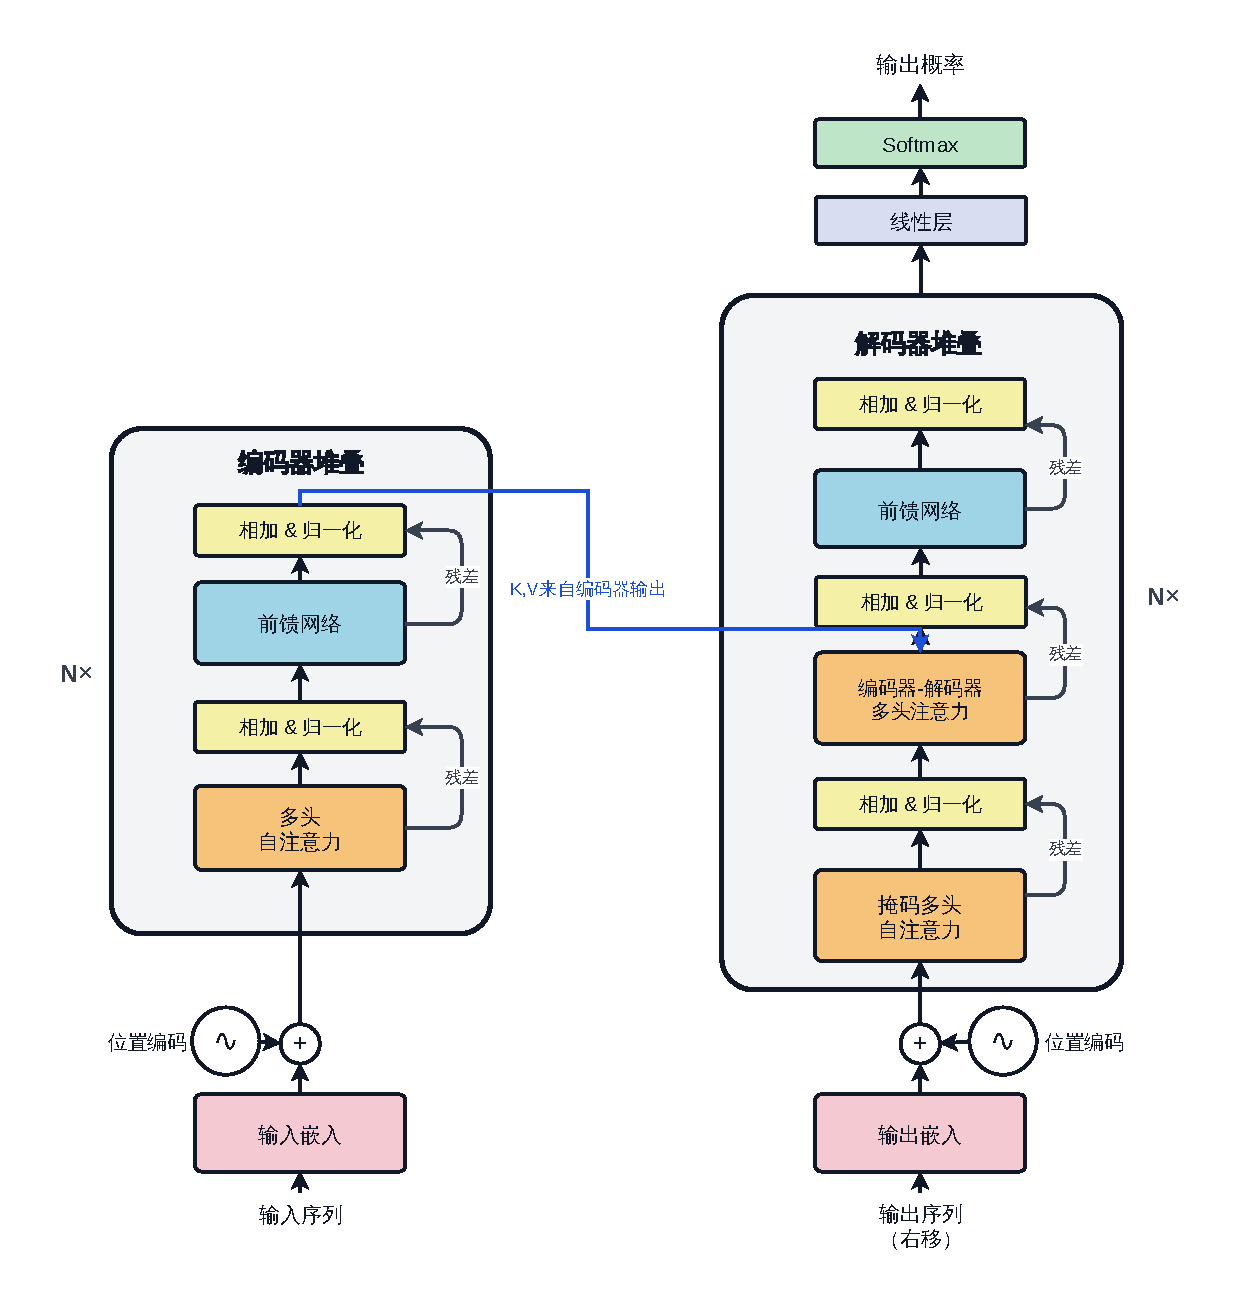
\includegraphics[width=0.70\textwidth]{images/feedback_diagrams/chapter3/transformer/transformer.drawio.pdf}
    \caption{参考原始Transformer结构重绘的编码器、解码器及语音情绪识别中编码器分类路径}
    \label{fig:transformer_full_architecture}
\end{figure}

图\ref{fig:transformer_full_architecture}在原始Transformer编码器-解码器结构基础上标出了语音情绪识别中的编码器分类路径。本文后续实验不使用生成式解码器。图中右侧路径用于说明编码器输出如何进一步进入池化或分类头。



\subsection{Transformer的整体架构}

Transformer模型基于编码器与解码器构成的堆叠结构。各编码器层与解码器层采用相同的内部结构重复堆叠，输入表示经过这些重复结构逐步转换为融合上下文信息的高维表示\cite{vaswani2017attention}。最初的Transformer模型针对序列到序列的转换任务提出，同时使用编码器和解码器。编码器从输入序列中提取上下文表示，解码器则参考编码器的输出逐步生成目标序列。

设输入表示为 $X \in \mathbb{R}^{T \times d}$，编码器依次通过多个编码器层，逐步反映输入序列的内部关系。这一过程可按层表示如下：
\begin{equation}
H^{(0)} = X
\label{eq:transformer_encoder_input}
\end{equation}
\begin{equation}
H^{(l)} = \mathrm{EncoderLayer}^{(l)}\!\left(H^{(l-1)}\right), \qquad l=1,2,\dots,L_e
\label{eq:transformer_encoder_stack}
\end{equation}
其中 $H^{(0)}$ 为编码器的初始输入表示，$H^{(l)}$ 为第 $l$ 个编码器层的输出，$L_e$ 为编码器层数。通过这种重复结构，输入序列中各个位置的表示逐渐融入更广的上下文信息\cite{vaswani2017attention}。

解码器接收目标序列或对应的中间表示作为输入，同时参考编码器的输出表示，逐步生成下一阶段输出。语音情绪识别通常是发话级分类任务，后续实验更关注编码器输出如何形成分类表示。解码器部分在本文中仅作为原始Transformer结构背景说明\cite{vaswani2017attention}。

Transformer可以在同一层内同时计算序列中多个位置之间的相关性，有利于并行计算，且无需像循环神经网络那样经过多个时间步的状态传递，也无需通过增加卷积层来扩大感受野，可以直接建模输入内部的全局关系\cite{vaswani2017attention,chen2023dwformer,wang2024swin}。

语音情绪识别通常是对整个发话进行分类的任务，原始Transformer的编码器-解码器结构常被简化为以编码器为中心的形式或进行适当变形\cite{chen2023dwformer,wang2024swin,ahn2025multitask}。在此情况下，可在编码器的最终输出上结合池化或分类头，进行发话级别的预测。该过程可概念性地表示为：
\begin{equation}
\hat{y} = \mathrm{Classifier}\!\left(\mathrm{Pool}\!\left(H^{(L_e)}\right)\right)
\label{eq:transformer_ser_prediction}
\end{equation}
其中 $\mathrm{Pool}(\cdot)$ 表示形成发话级表示的操作，如平均池化、注意力池化或基于分类标记的聚合等，$\hat{y}$ 为最终的预测情绪类别。近年来，在语音情绪识别研究中，人们提出在以编码器为中心的结构之上，结合基于窗口的注意力、分层补丁表示或与卷积神经网络混合的结构，以调整计算范围和表示单元\cite{liu2023dualrobustness,chen2023dwformer,wang2024swin,ahn2025multitask}。

\subsection{位置编码机制}

Transformer的注意力运算适合计算输入向量之间的相关性，但注意力运算本身不反映序列的顺序。当给定一组相同的输入向量时，若未提供位置信息，模型难以从结构上区分位置1与位置10的差异。在原始Transformer模型中，通过在输入嵌入中加入位置编码来缓解位置信息的缺失\cite{vaswani2017attention}。

较为常见的固定型位置编码使用正弦函数和余弦函数为每个位置构造对应的向量。设位置索引为 $pos$，维度索引为 $i$，总维度为 $d$，固定型位置编码通常可定义为\cite{vaswani2017attention}：
\begin{equation}
PE(pos,2i)=\sin\left(\frac{pos}{10000^{2i/d}}\right)
\label{eq:pe_sin}
\end{equation}
\begin{equation}
PE(pos,2i+1)=\cos\left(\frac{pos}{10000^{2i/d}}\right)
\label{eq:pe_cos}
\end{equation}
其中偶数维度使用正弦函数，奇数维度使用余弦函数。这种构造方式利用不同周期的周期函数，以连续形式表示各个位置。当位置距离发生变化时，各维度的变化模式也随之不同，模型可同时利用绝对位置信息以及位置之间的相对差异信息\cite{vaswani2017attention}。

设输入表示为 $X \in \mathbb{R}^{T \times d}$，位置编码矩阵为 $PE \in \mathbb{R}^{T \times d}$，融合位置信息后的最终输入可表示为：
\begin{equation}
X' = X + PE
\label{eq:pe_add}
\end{equation}
其中 $X'$ 为补充位置信息后的输入表示。通过这种加法结构，原始输入特征与位置信息在同一维度空间中共同传递。后续注意力运算除了比较各位置的特征值，还计算包含位置信息的表示之间的相关性\cite{vaswani2017attention}。


除固定型位置编码外，也可将位置向量作为可学习参数在训练中直接更新，但其行为可能受训练数据长度分布影响，对未见长度序列的推广能力与固定型方法有所不同\cite{vaswani2017attention}。

在语音情绪识别中，位置编码的含义与自然语言处理存在差异。自然语言处理中通常反映单词或子词标记的顺序，语音情绪识别中的输入单元往往是对数梅尔谱图的帧序列、梅尔频率倒谱系数序列或基于补丁的频谱表示\cite{chen2023dwformer,wang2024swin,ahn2025multitask}。在此情况下，位置编码用于表示每个帧或每个补丁在发话中的时间位置。即使相同的频率结构出现，该频率结构出现在发话早期、中期还是后期，其情绪含义可能不同。补充位置信息可视为反映时间序列结构的一个因素。



\subsection{ Transformer层中的关键组成结构}

Transformer的编码器和解码器由注意力子层堆叠而成。Transformer的一层由注意力运算和用于表示重组、层间信息传递稳定的补充结构共同构成。在原始Transformer中，每个注意力子层之后依次应用残差连接与层归一化，随后放置位置级前馈网络，之后再次应用残差连接与层归一化\cite{vaswani2017attention}。

以一个编码器层为例，输入表示 $H^{(l-1)}$ 首先经过多头自注意力子层，该子层的输出通过残差连接与层归一化更新为中间表示 $\tilde{H}^{(l)}$。这个中间表示随后通过位置级前馈网络，再次经过残差连接与层归一化，形成最终输出 $H^{(l)}$。该过程可表示为：
\begin{equation}
\tilde{H}^{(l)} = \mathrm{LayerNorm}\!\left(H^{(l-1)} + \mathrm{MHA}\!\left(H^{(l-1)}\right)\right)
\label{eq:encoder_mha_block}
\end{equation}
\begin{equation}
H^{(l)} = \mathrm{LayerNorm}\!\left(\tilde{H}^{(l)} + \mathrm{FFN}\!\left(\tilde{H}^{(l)}\right)\right)
\label{eq:encoder_ffn_block}
\end{equation}
其中 $\mathrm{MHA}(\cdot)$ 表示该编码器层的多头自注意力子层，$\mathrm{FFN}(\cdot)$ 表示位置级前馈网络。在编码器层内部，首先通过自注意力反映同一输入序列内部的相关性，随后各位置的表示独立经过非线性变换，形成最终输出\cite{vaswani2017attention}。

\begin{figure}[htbp]
    \centering
    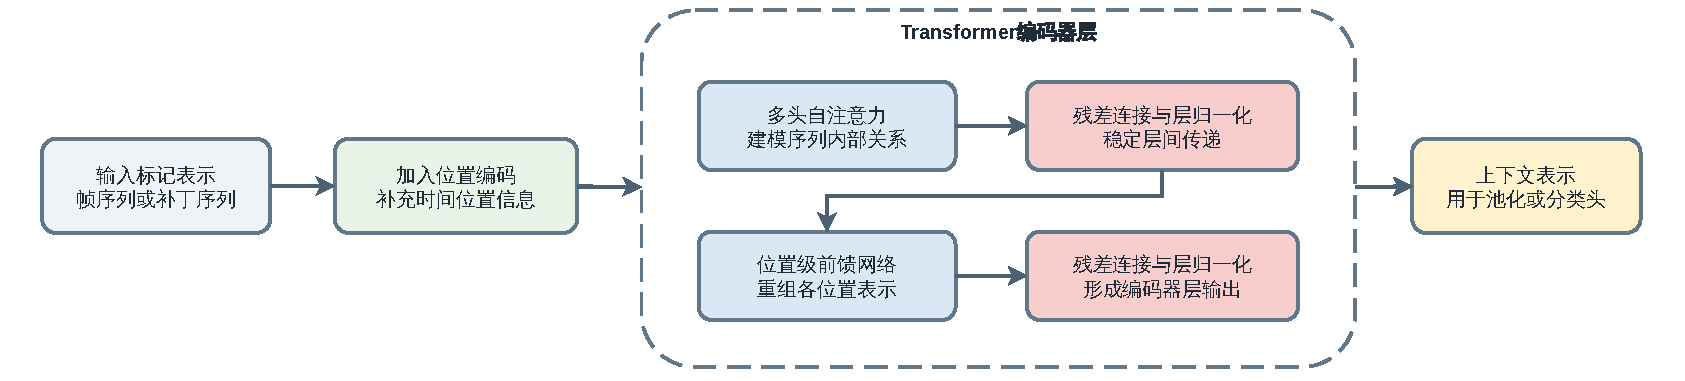
\includegraphics[width=0.68\textwidth]{images/chapter3/chapter3_transformer_encoder.drawio.pdf}
    \caption{Transformer编码器层的基本信息流动}
    \label{fig:chapter3_transformer_encoder}
\end{figure}

图\ref{fig:chapter3_transformer_encoder}对应上述编码器层公式，展示输入标记表示加入位置编码后，依次经过多头自注意力、残差连接、层归一化和位置级前馈网络的过程。该流程说明编码器层如何在同一序列内部整合上下文。同时保持层间表示稳定。

解码器层的内部结构与编码器层相近，但额外包含掩码多头自注意力和编码器-解码器注意力。前者限制未来时刻信息直接参与，后者使解码器表示参考编码器输出。本文实验未采用生成式解码路径，后文重点放在编码器层、位置编码、残差连接、层归一化和位置级前馈网络等与分类模型关系更直接的结构上\cite{vaswani2017attention}。

位置级前馈网络的作用是将注意力形成的上下文信息在各位置表示层面进行再变换。这种网络对已通过注意力融入上下文信息的每个位置向量施加相同的非线性变换。该网络不直接计算序列中不同位置之间的关系。其一般形式为：
\begin{equation}
\mathrm{FFN}(x) = W_2\,\sigma(W_1x + b_1) + b_2
\label{eq:ffn_general}
\end{equation}
其中 $x$ 为某一位置的输入向量，$W_1$、$W_2$ 为权重矩阵，$b_1$、$b_2$ 为偏置向量，$\sigma(\cdot)$ 为非线性激活函数。该步骤可视为在注意力聚合的上下文信息基础上对每个位置表示进行进一步重组\cite{vaswani2017attention}。

残差连接将子层的输入表示直接加到变换结果上。其一般形式为：
\begin{equation}
y = x + \mathcal{F}(x)
\label{eq:residual_general}
\end{equation}
其中 $x$ 为子层输入，$\mathcal{F}(x)$ 为经过注意力或前馈网络后的变换结果。残差连接在保留原始输入信息的同时加入变换结果，有助于缓解深层网络中信息过度衰减的问题\cite{vaswani2017attention}。

层归一化对每个位置表示向量内部的各维度计算均值 $\mu$ 和方差 $\sigma^2$，并通过可学习参数 $\gamma, \beta$ 进行尺度归一化：
\begin{equation}
\mathrm{LayerNorm}(x)=\gamma \odot \frac{x-\mu}{\sqrt{\sigma^2+\epsilon}}+\beta
\label{eq:layernorm_general}
\end{equation}
其中 $\epsilon$ 为防数值不稳定的小常数。层归一化在每个位置的表示向量内部进行归一化，对序列长度和批次大小的变化相对不敏感\cite{vaswani2017attention}。





\subsection{ Transformer的主要特点及其适用边界}

Transformer通过自注意力机制可以同时计算多个位置之间的相关性，有利于并行计算，并能够直接建模输入内部的全局关系\cite{vaswani2017attention}。在语音情绪识别中，情绪信息可能分布在发话的多个时刻，这种全局建模特性与发话级分类任务具有一定的相关性\cite{chen2023dwformer,wang2024swin}。

Transformer的稳定性受数据规模和任务条件影响。随着输入长度增加，计算量和内存占用可能相应增加，实际研究中已提出基于窗口的注意力、移位窗口、分层补丁表示等结构调整方法\cite{chen2023dwformer,wang2024swin}。语音情绪识别数据通常规模不大，在此类条件下，结构复杂的模型可能同时学习到情绪相关模式以及数据集本身的偏差，近年来研究者提出调整输入范围或结合多任务学习等方式加以应对\cite{chen2023dwformer,wang2024swin,ahn2025multitask}。

\begin{figure}[!t]
    \centering
    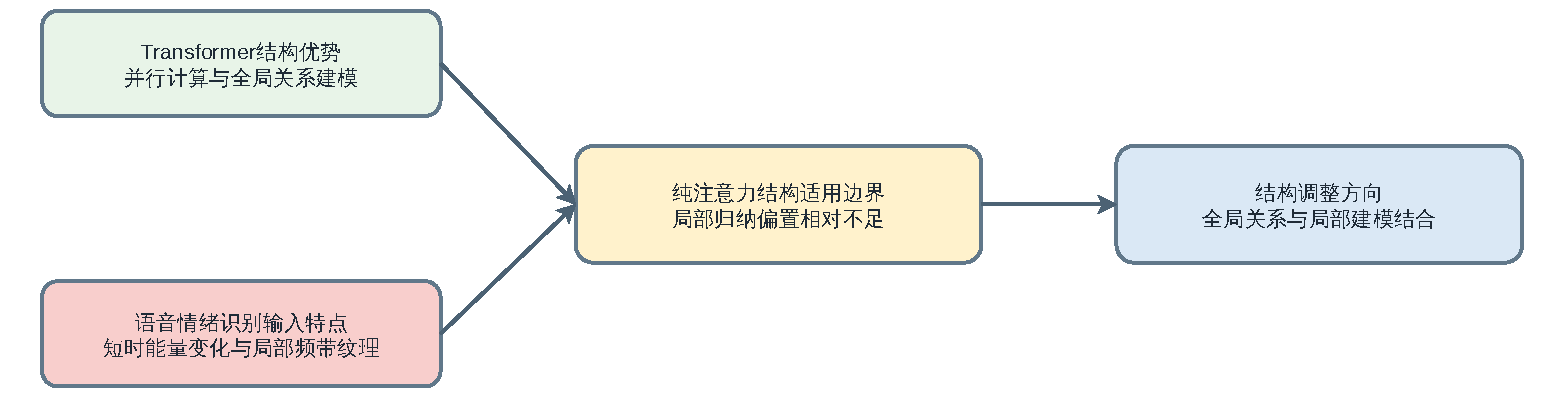
\includegraphics[width=0.72\textwidth]{images/chapter3/chapter3_transformer_ser_boundary.drawio.pdf}
    \caption{Transformer在语音情绪识别中的适用边界}
    \label{fig:chapter3_transformer_ser_boundary}
\end{figure}



\section{本章小结}

本章围绕语音情绪识别模型结构展开说明，依次介绍了基础神经网络模型、注意力机制和Transformer结构。前馈神经网络能够处理固定维度特征表示，但对语音序列中的局部时频模式和长时依赖关系刻画较为有限。卷积神经网络通过局部感受野和参数共享机制提取二维谱图中的局部模式，在对数梅尔频谱输入条件下具有较好的结构适配性。循环神经网络、长短时记忆网络和门控循环单元则从时间递推角度处理序列信息，为语音情绪识别中的时序建模提供了基础方案。

在注意力机制部分，本章说明了注意力得分、权重归一化和加权求和的基本过程，并进一步讨论了自注意力、多头注意力以及注意力池化等结构。注意力机制的作用在于根据输入内部不同位置之间的相关性重新分配信息权重，使模型能够从发话中筛选与情绪判断关系较大的片段。对于语音情绪识别任务，注意力机制既可作为序列编码器内部的关系建模方式，也可作为发话级表示聚合方法。

在Transformer结构部分，本章介绍了编码器结构、位置编码、残差连接、层归一化和位置级前馈网络等组成部分。Transformer通过自注意力机制计算序列内部不同位置之间的关系，适合刻画较长范围的上下文信息；但在语音情绪识别这类数据规模相对有限的任务中，纯注意力结构也可能面临局部声学线索不足和训练稳定性不足的问题。基于上述分析，第四章将卷积神经网络基线模型、纯Transformer模型和CNN-Conformer模型作为主要比较对象，用实验结果检验局部时频建模、全局上下文建模以及二者组合后的表现差异。
